\documentclass[]{article}
\usepackage[margin=1.1in, portrait]{geometry}
%\usepackage{fullpage}
\usepackage{amsmath}
\usepackage{amssymb}
\usepackage{amsthm}
\usepackage{mathrsfs}
\usepackage[english]{babel}
\usepackage{multirow}
\usepackage{graphicx}
\newtheorem{stel}{Stelling}
\usepackage{float}
\usepackage{textcomp}
\usepackage{footmisc}
\usepackage[colorlinks=true, urlcolor=blue, linkcolor=blue, citecolor=blue, pdfborder={0 0 0}, linktoc=page]{hyperref}
\setlength{\parindent}{0 pt}
\usepackage{etoolbox}
\usepackage{scrextend}

\newcommand{\ba}{\begin{addmargin}[9mm]{0cm}}
\newcommand{\ea}{\end{addmargin}}
\newcommand{\cm}{\color{blue} \hspace{3mm}}



\title{
  \begin{figure}[H]
	   \centering
	   
\includegraphics[scale=.3]{Images/Magritte_logo_v2_BW.pdf}
  \end{figure}
  \vskip-3mm
  \textsc{\Large MAGRITTE: Multidimensional Accelerated General-purpose RadIaTive TransfEr}   \\
  \vskip13mm
  \textsc{\Huge Code Documentation}
}

\author{\Large \vskip13mm Frederik De Ceuster}
\date{}



\begin{document}

\maketitle

\vskip13mm

\begin{abstract}
This report gives an overview of some technical aspects of the Magritte code. The goal is to motivate why and explain how some things are coded the way they are.
\end{abstract}


\newpage

\tableofcontents


\newpage


\section{General}

Magritte is a multipurpose accelerated 3D radiative transfer code. Given a gas with a density and velocity distribution, an external radiation field and a provisional chemical composition, it selfconsistently calculates the temperature, level populations and chemical composition of the gas. Magritte is a ray-tracing code, meaning that to solve for the transport of electromagnetic radiation, the radiative transfer equation is solved along a set of rays.

\bigskip

The first version of Magritte is mainly based on 3D-PDR \cite{3DPDR}. The main difference is that in Magritte the radiative transfer is solved exactly and not in the Sobolev or large velocity gradient (LVG) approximation.

\bigskip

The code is mainly written in C with some features of C++. For the ray tracing the discretization scheme of the unit sphere is used from HEALPix\footnote{\url{https://healpix.jpl.nasa.gov}}. The chemical rate equations are solved using the CVODE solver provided in SUNDIALS\footnote{\url{https://computation.llnl.gov/projects/sundials}}. Most of the linear algebra is done using the Eigen\footnote{\url{http://eigen.tuxfamily.org}} library.



\section{Some structures}

\subsection{(HEALPix) rays}

To model the propagation of light through the grid, we need to trace rays through it i.e. determine which grid points you pass when you travel along a straight line in a certain direction. The first step is to discretize all directions. This is done using HEALPix. The algorithm considers a unit sphere and devides it into \texttt{NRAYS} segments. Afterwards it asigns unit vectors from the center of the sphere to the center each segments. These vectors form a discretization of all directions in 3D space. To facillitate the calculations of the radiative transfer, we require a discretization in which for each ray there is an antipodal ray (i.e. a ray in the oposite direction). This can be obtained by demanding that the \texttt{NRAYS} is of the form $12n^{2}$ where $n$ is an integer. We consider \texttt{NRAYS} rays (as defined by the HEALPix vectors) around each grid point.

\begin{figure}[H]
	\centering
	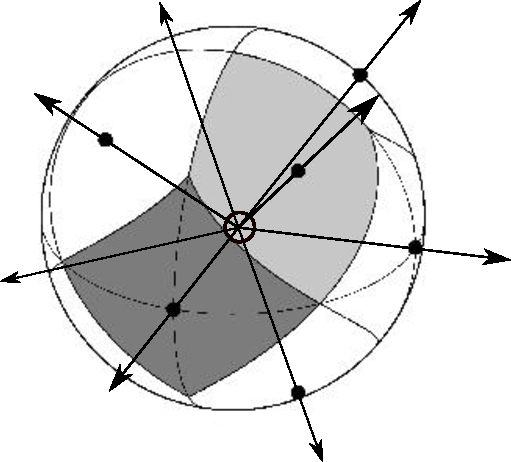
\includegraphics[scale=.7]{Images/healpixrays.pdf}
	\caption{HEALPix rays through segment centers that discretize the sphere.}
	\label{grid}
\end{figure}

\subsection{New types \texttt{GRIDPOINT}, \texttt{EVALPOINT}, \texttt{SPECIES} and \texttt{REACTION} }
The code defines four new types: \texttt{GRIDPOINT}, \texttt{EVALPOINT}, \texttt{SPECIES} and \texttt{REACTION}. Each of these represents a type of objects that is used extensively in the code.

\begin{equation}
\texttt{GRIDPOINT gridpoint.}
\begin{cases}
\ \texttt{double x, y, z} & \text{position}\\
\ \texttt{double vx, vy, vz} &  \text{gas velocity} \\
\ \texttt{double density} &  \text{gas density} \\
\end{cases}
\end{equation}

\texttt{GRIDPOINT} stores all informtion that comes with the input gird. This includes the three components of the position vector of the grid point, the three components of the velocity and the density of the gas at that point. These parameters are the typical output of a hydrodynamical simulation. As one could expect, there is one \texttt{GRIDPOINT} object for each point in the gird.

\begin{equation}
\texttt{EVALPOINT evalpoint.}
\begin{cases}

\end{cases}
\end{equation}

\texttt{EVALPOINT} represents the so-called evaluation points which store the information on the rays passing through the grid points.  An evaluation point is the projection of a grid point on a ray. Since integrations are often done along a ray, the physical quantities are evaluated at the projections of the grid points these rays. Hence the name: evaluation points. The most important parameters stored for an evaluations points are the distance between consecutive points and the projection of the gas velocity along the ray. For every grid point we have a set of rays. Ideally every other grid point lies on one of such rays. As a result we have (maximally) $\texttt{NGRID}*\texttt{NGRID}$ evaluation points.

\begin{equation}
\texttt{SPECIES species.}
\begin{cases}
\ \texttt{string sym} & \text{chemical symbol}\\
\ \texttt{double mass} & \text{molar mass} \\
\ \texttt{double abn[NGRID]} &  \text{abundance} \\
\end{cases}
\end{equation}

\texttt{SPECIES} stores the properties of a chemical species. These include the symbol of the species, its abundance and its molar mass. All this data is read by the function \texttt{read\_species} in the \texttt{read\_chemdata.cpp} file.

\begin{equation}
\texttt{REACTION reaction.}
\begin{cases}
\ \texttt{string R1, R2, R3} & \text{symbols of reactants}\\
\ \texttt{string P1, P2, P3, P4} & \text{symbols of reaction products} \\
\ \texttt{double alpha, beta, gamma} &  \text{parameters determining reaction rate} \\
\ \texttt{double RT\_min, RT\_max} &  \text{temperature range where parameters apply} \\
\ \texttt{double k[NGRID]} &  \text{reaction rate at every grid point} \\
\ \texttt{int    dup} &  \text{number of duplicates in other T ranges}
\end{cases}
\end{equation}

\texttt{REACTION} contains the information on the chemical reactions. There is place for three reactants and four reaction products. For each of those the symbol of the species is stored. Furthermore there are three constants \texttt{alpha}, \texttt{beta} and \texttt{gamma} which will determine the reaction rate, and two temperatures giving the range where these constants apply. All parameters mentionned above are read by the \texttt{read\_reactions} function in the \texttt{read\_chemdata.cpp} file. Finally also the reaction rate is stored after it is calculated in the \texttt{reaction\_rates} function.


\subsection{Storing multi-dimensional arrays as lists}

All multi-dimensional arrays in the code are stored as one-dimensional lists. On the lowest level, this is the case in every computer code. However, we chose to explicitly write the one-dimensional lists and define the relations between list index and the rows and columns.

\section{Ray tracing}

To be able to simulate 3-dimensional objects we need a way to represent them in computer language. In this first verison of the code space is dicretized into a truely unstructered grid. In a truely unstructered grid every point is stored separately, without any relation between different points. Physical quantities as the position, gas velocity and temperature are stored independent for every point. In a later version we aim to exploit more the possible structure of the grid.

\bigskip

Space is discretized into \texttt{ngrid} grid points.

\subsection{Efficiently storing the evaluation points}

THE ORIGIN IS NOT AN EVALUATION POINT!

\texttt{raytot[RINDEX(n,r)]} gives the total number of evaluation points on a ray \texttt{r} through a gridpoint \texttt{n}. Here the origin is not counted as an evaluation point. Otherwise we would store the origin each time as an evaluation point, resulting in \texttt{ngrid} times \texttt{NRAYS} unnecessary doubles. In the radiative transfer part of the code we do want to consider the origin as an eveluation point. Therefore we will systematically add one to \texttt{raytot} in that part of the code.

\subsection{Equivalent rays}
of

\section{Radiative transfer}

\begin{figure}[H]
	\centering
	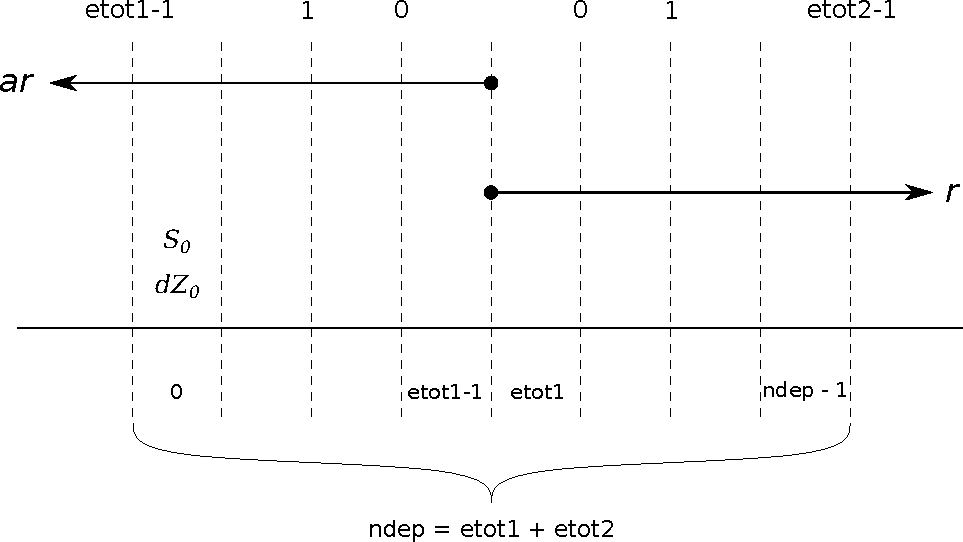
\includegraphics[scale=.8]{Images/ray.pdf}
	\caption{Construction of the ray along wich the radiative transfer is solved.}
	\label{grid}
\end{figure}


\subsection{\texttt{exact\_feautrier} solver}

Based on the benchmarks, we can conclude that the \texttt{exact\_feautrier} solver has a 9 digit precission.


\newpage

\bibliography{library}
\bibliographystyle{ieeetr}



\end{document}
